\chapter{Implementación}

\section {Unidades del proyecto}
El proyecto consistente en una aplicación para la gestión de entrenamientos se compone de dos partes claramente diferenciadas, el backend y el frontend.
\begin{itemize}
  \item \textbf{Frontend:} El frontend es la aplicación web (\gls{SPA} - Single Page Application) con la que los usuarios finales interactúan, en ella se proporciona una autenticación mediante los servicios de Google, Facebook y usuario/contraseña, formularios para la introducción de datos, y visualizaciones para las progresiones y los entrenamientos. El frontend se ha desarrollado haciendo uso de React, apoyado en diversos paquetes, entre los que cabe destacar Redux, React-Router, Chart.js, Material UI y Redux-Forms.
  \item \textbf{Backend:} El backend, también programado completamente en javascript, es la parte encargada de proporcionar y almacenar los datos del frontend. En este caso es dicho backend es una API RESTful, creada sobre Node.js y el paquete Express. Como base de datos se usa una base de datos MongoDB debido a su flexibilidad y a su rendimiento. Para la interacción entre Node y el servidor de DB, hacemos uso de un famoso paquete llamado Mongoose, que destaca por su capacidad para hacer consultas complejas de una forma sencilla. Ademas de esto existe un sistema de \gls{logging} llamado Papertrail, el cual nos permite obtener estadísticas acerca de las peticiones realizadas a nuestra API.
\end{itemize}

\section {Tecnologías y herramientas}
\subsection {Tecnologías}
En este Apartado vamos a comentar las tecnologías usadas para el desarrollo, centrándonos en la pila MERN, y destacando alguno de los paquetes más relevantes. La pila anteriormente mencionada se compone de MongoDB, ExpressJS, React JS y Node JS.
\begin{itemize}
  \item \textbf{MongoDB:} Mongo es un sistema de base de datos de código abierto, es un sistema No-SQL orientado a documentos, dichos documentos tienen un formato llamado \gls{BSON}, muy similar a \gls{JSON}, lo cual hace su integración con javascript muy sencilla. Además se puede usar javascript como lenguaje de consultas, haciendo que todo el proyecto tenga un código homogéneo. Hemos decido hacer uso de este motor de bases de datos debido a su gran comunidad, y además hemos optado por una No-SQL en lugar de por ejemplo MySQL debido a que los esquemas de los datos irían evolucionando a lo largo del tiempo y su modificación es muy simple con MongoDB.
  
  \item \textbf{Express JS:} Express es una capa que corre sobre Node, para facilitar la creación APIs, siendo el framework más usado para este propósito, y de hecho considerado el estándar de facto para la creación de APIs con Node. Tras valorar otras alternativas como Hapi o Koa, decidimos que esta era la opción más conveniente debido a su rendimiento y amplia comunidad.
  
  \item \textbf{ReactJS:} React es una biblioteca de Javascript diseñado para el desarrollo de aplicaciones de solo una pagina. El desarrollo con esta tecnología, se basa en la creación de pequeños componentes reutilizables, que mediante su combinación haciendo uso del lenguaje \gls{JSX}, crean componentes mayores. Esta fue una de las decisiones mas complejas, ya que de ella dependería todo el diseño del frontend. Tras valorar Angular y React, decidimos optar por esta ultima ya que es muy ligero, eficiente, modular y eficiente, aunque su ligereza añade cierta complejidad a la hora de elegir los paquetes, ayuda a obtener una personalización y adaptación máxima al proyecto.
  
  \item \textbf{NodeJS:} Node es un servidor para la ejecución de javascript basado en el motor V8 de chrome. 
\end{itemize}

Alguno de los paquetes más relevantes son:
\begin{itemize}
  \item \textbf{React-Router-Dom:} React-Router-Dom es el paquete que se encarga del mapeo de las URL a los componentes de React, además tiene la característica de que es capaz, con la implementación correcta, de crear una navegación entre diferentes partes de la aplicación web sin necesidad de recarga, pro
proporcionando una sensación más similar a una aplicación de escritorio.

  \item \textbf{Redux:} Redux, quizá sea el paquete más relevante a la hora de trabajar con React, proporcionando una forma para centralizar el estado de todos los componentes, de forma que es una "fuente de verdad", de la que todos los componentes leen su estado, con lo cual se crea una fácil comunicación entre los diferentes componentes, evitando problemas de sincronización entre ellos. Se decidió hacer uso de este en lugar de Mobx debido a que se trata del estándar de facto, por lo que incluye una mayor comunidad y una gran documentación.
  
  \item \textbf{Material UI:} Material UI es un paquete que nos proporciona una serie de estilos y componentes ayudándonos con la creación de web con un estilo consistente. Tras valorar alternativas como adaptaciones de Bootstrap, la amplia cantidad de componentes disponibles y el diseño "Material design" predefinido hizo que nos inclináramos por esta.
  
  \item \textbf{Mongoose:} Mongoose es un \gls{ODM} que nos permite tratar las consultas y las colecciones de MongoDB como objetos, dando la posibilidad de crear complejas consultas de una forma sencilla. Aunque podíamos hacer uso del \gls{driver} nativo de MongoDB, la simplicidad y las herramientas añadidas como los "\gls{pseudojoins}" hizo que pareciera una decisión más acertada el uso de este ODM.
  
  \item \textbf{Auth0-Lock:} Este paquete, nos ayuda con la integración con Auth0, que es un servicio para la administración de identidades y autenticación. Aunque podríamos haber realizado la integración manualmente o con soluciones como Passport, decidimos optar por el paquete oficial para evitar posibles incompatibilidades en el momento de las actualizaciones.
  
\end{itemize}
\subsection {Herramientas}
En esta subsección haremos una breve descripción de algunas de la herramientas usadas para la compilación, despliegue y verificación de la calidad del código.

\begin{itemize}
  \item \textbf{Docker:} Es una tecnología para la creación, administración y uso de contenedores de Linux. Dichos contenedores nos proporcionan la ventaja de evitar tener ciertas redundancias que se crean con el uso de máquinas virtuales.
  
  \item \textbf{Ansible:} Ansible es una plataforma para configurar y administrar computadoras, este tipo de software, se conoce como software de \gls{orquestacion}, y en nuestro caso lo usamos para provisionar y configurar las máquinas virtuales creadas en la nube de Google.
  
  \item \textbf{Webpack:} Webpack es un empaquetador de módulos, usado para crear el "\gls{bundle}" con la aplicación web, aunque dispone de múltiples funciones avanzadas, que se mostrarán en el anexo, su objetivo principal es agrupar los archivos de JavaScript para su uso en un navegador, pero también es capaz de transformar, agrupar o empacar casi cualquier recurso. Decidimos hacer uso de este en lugar Gulp o Grunt, debido a su gran comunidad y cantidad de plugins para la optimización de código React entre otras cosas.

  \item \textbf{Jest:} Jest es el paquete que usaremos para la implementación de los test unitarios y los test de cobertura. También han sido considerados paquetes como Mocha y Chai, pero debido a que este paquete integra toda la funcionalidad de ambos, además de algunas funciones extra, decidimos optar por el.
  
  \item \textbf{NPM:} NPM es el gestor de paquetes de Node, desde el cual obtendremos y administramos todas las dependencias de nuestro proyecto. Podríamos haber optado por Yarn que funciona como una capa sobre NPM, pero aunque en el pasado esto podría haber tenido sentido, la evolución de NPM hace que no sea necesario.
  
  \item \textbf{Auth0:} Auth0 es una solución para la gestión de la autenticación y los usuarios de un servicio web, el cual nos permite una integración sencilla con la autenticación de otros proveedores como Google o Facebook.  Gracias a ello nos despreocupamos de la delicada gestión de las contraseñas de usuario, correos de recuperación, confirmación, integración con otros servicios... que aunque se puede hacer manualmente añade bastante complejidad.
  
  \item \textbf{Vagrant:} Vagrant es una herramienta para la creación y configuración de entornos de desarrollo virtualizados.
  
  \item \textbf{Fabric: } Fabric es una biblioteca de python para la ejecución de comandos en remoto, dándonos la posibilidad de administrar nuestros servidores en la nube de una forma sencilla.
  
  \item \textbf{PM2:} PM2 es un gestor avanzado de procesos de Node, que nos permitirá, iniciar y parar procesos, reiniciar, mantenerlos siempre activos evitando caídas, reinicios sin tiempo de caída, balanceo de carga... Aunque había otras alternativas como Forever, debido a su simplicidad, su gran comunidad y la posibilidad de escalar las aplicaciones, nos hizo decidirnos por PM2
  
  \item \textbf{NGINX:} En esta aplicación y solo para el despliegue en Google Cloud, usaremos Nginx en modo \gls{proxy inverso}.
  
  \item \textbf{Nodemon:} Nodemon es un servicio que monitoriza los cambios en los archivos y reinicia el servidor de node automáticamente, lo cual es muy útil durante el desarrollo.
  
  \item \textbf{mLab:} mLab es un servidor de bases de datos Mongo en la nube, en el cual guardaremos los datos de la app. Debido a su fácil configuración, que nos evita tener que crear un servidor y que es gratuito, optamos por esta solución.
  
  \item \textbf{PaperTrail:} PaperTrail es un sistema para administrar datos de logs de nuestra app de forma sencilla, mediante los cuales podremos obtener información útil como los endpoints más usados y los tiempos de respuesta del servidor.
  
  \item \textbf{Git/GitHub:} Git es un sistema de control de versiones que nos permite desarrollar el código de una forma fiable y con posibilidad de revertir cambios si es necesario. Existen también otros sistemas de control de versiones como Mercurial, pero debido a la popularidad y la gran cantidad de integraciones, \gls{git} fue la mejor opción.
  
  \item \textbf{GreenKeeper:} Greenkeeper es una herramienta que monitoriza el archivo package.json, que es donde se encuentran todas las dependencias de proyecto, de forma que es capaz de crear nuevas ramas y solicitar un pull request cuando aparecen nuevas versiones de las dependencias, proporcionando información sobre si se pasan los test y los cambios y nuevas características de la versión.
  
  \item \textbf{David-dm:} Es otro sistema para mantenernos al tanto de actualizaciones en las dependencias del proyecto.
  
  \item \textbf{Husky:} Husky es una herramienta que nos permite configurar \gls{hooks} para Git, en nuestro caso está configurada para garantizar que todo el código subido al repositorio se ajusta al mismo estilo, mediante el uso de Prettier y la guía de estilos de AirBnB.
  
  \item \textbf{Prettier:} Prettier es un formateador de código, para mantener un formato coherente en toda la app. 
  
  \item \textbf{ESlint:} ESLint es un "\gls{linter}" para javascript, que nos ayuda a mantener la calidad del código durante el desarrollo.
  
  \item \textbf{SonarQube:} SonarQube es una herramienta online, que es capaz de analizar nuestro código en busca de bugs, código de baja calidad, código repetido...
  
  \item \textbf{Travis CI:} Travis CI es un sistema de integración continua, durante el desarrollo, nos apoyaremos en él para los despliegues automáticos y la fusión de nuevas ramas en el repositorio de Git.
  
  \item \textbf{Heroku:} Heroku es un \gls{PaaS} (Platform as service), en el cual se llevará a cabo un despliegue continuo, de forma que seremos capaces de desplegar nuevas características de la App de una forma rápida, sencilla y sin tiempos de caída.

\end{itemize}
\section {Test unitarios y de cobertura}
\subsection {Test Unitarios}
Para la realización de los test unitarios, hemos adaptado una metodología enfocada a la evaluación de los comportamientos deseados, para ello hemos hecho uso de la herramienta Jest, las cual nos permite describir test de forma que se evalúa el éxito o el fracaso dependiendo de si obtenemos el resultado deseado o no, un ejemplo de la implementación de estos test, se puede ver en el siguiente fragmento de código. Se pueden encontrar más ejemplos en \url{https://github.com/antoniovj1/tfg_gymapp/tree/master/__tests__}
\begin{lstlisting}[language=javascript,caption={Test Unitarios},label={lst:appjs}]
//.....

describe('Exercise (/api/training/exercise/)', () => {
  let server;
  const user = new User({ auth0id: 'ex' });

  beforeAll(async () => {
    server = require('../../server');

    await Exercise.remove({});
    await Session.remove({});
    await Movement.remove({});
    await User.remove({});
    await user.save();
  });

  afterAll(async () => {
    try {
      await Exercise.remove({});
      await Session.remove({});
      await Movement.remove({});
      await mongoose.disconnect();
      await server.shutdown();
    } catch (error) {
      throw error;
    }
  });

  describe('/GET/:id_exercise', () => {

    test('should fail with incorrect id', done => {
      const exercise = new Exercise();

      exercise.save((err, exercise) => {
        chai
          .request(server)
          .get('/api/training/exercise/' + 'ididididid')
          .set('x-access-token', token)
          .end((err, res) => {
            expect(res.status).toBe(200);
            expect(res.body).toHaveProperty('message', 'fail');
            done();
          });
      });
    });
  });
});
\end{lstlisting}
\subsection { Test de cobertura }
Los test de cobertura son una serie de test que nos permiten conocer qué porcentaje del codigo esta testeado, en este caso y gracias a Jest, no se requiere de ninguna implementación especial, ya que haciendo uso de los test de unitarios es capaz de identificar qué partes del código han sido usadas para los test y cuales no, proporcionando información de porcentaje testeado, líneas no testeadas, funciones no testeadas o archivos no testeados.

Los comandos requeridos para ejecutar los test, están definidos en archivo package.json que es el usado por NPM.
\lstset{
    string=[s]{"}{"},
    stringstyle=\color{blue},
    comment=[l]{:},
    commentstyle=\color{black},
}
\begin{lstlisting}
"scripts": {
    "build": webpack --config ./webpack.config.js --display-error-details --colors",
    "dev-server": "nodemon --config nodemon.json server.js",
    "postinstall": webpack --config ./webpack.config.js --display-error-details --colors",
    "start": node server.js",
    "test": "export SECRET='secret' && jest --verbose --forceExit --runInBand --silent",
    "test-cov": "export SECRET='secret' && jest --verbose --coverage --forceExit --runInBand --silent",
    "precommit": "lint-staged"
  },
\end{lstlisting}

\section {Integración continua y despliegue continuo}
\subsection{Integración continua}
Para la integración continua hemos optado por la solución Travis CI, lo cual hace realmente simple su implementación. Simplemente debemos registrarnos en la web de Travis, añadir nuestro repositorio y seleccionar las reglas que activan una nueva ejecución de nuestra batería de tests, en nuestro caso lo configuramos para ejecutarse en los push y en los merge. Además de esto debemos añadir un sencillo script de configuración a nuestro repositorio, en el cual se indica a Travis el entorno que debe preparar. El archivo de configuración es como se muestra a continuación:
\begin{lstlisting}[language=javascript,caption={Integración continua},label={lst:appjs}]
language: node_js
node_js:
  - "node"

services:
  - mongodb

cache:
  directories:
    - "node_modules"

\end{lstlisting}
\subsection {Despliegue continuo}
Para el despliegue continuo se ha optado por el uso de Heroku, un sistema que permite la integración con GitHub y Travis CI, y que ha sido configurado para crear la base de datos en mLab y de forma que con cada push a la rama master del repositorio que pasa los test, se crea un nuevo build y un despliegue automáticamente. Adicionalmente hemos creado un archivo de configuración de Heroku que permite el despliegue de la aplicación con un solo click de ratón.
\lstset{
    string=[s]{"}{"},
    stringstyle=\color{blue},
    comment=[l]{:},
    commentstyle=\color{black},
}
\begin{lstlisting}
{
  "name": "TFG UGR - GymApp",
  "description": "TFG",
  "website": "https://github.com/heroku/node-articles-nlp",
  "repository": "https://github.com/antoniovj1/tfg_gymapp",
  "logo": "https://node-js-sample.herokuapp.com/node.svg",
  "success_url": "/",
  "keywords": [
    "node",
    "express"
  ],
  "addons": [
    "mongolab"
  ]
}
\end{lstlisting}
\section {Provisionamiento, Cloud y Contenedores}
Además de la solución anterior para el despliegue en Heroku, también se han creado otros archivos de configuración para el despliegue en la nube y para el uso de contenedores.

\subsection {Provisionamiento}
El provisionamiento consiste en añadir todos los recursos y configuraciones a una máquina, para que la aplicación que queremos correr pueda funcionar correctamente y sin intervención de un usuario, en nuestro caso hemos hecho uso de Ansible, una herramienta que permite la configuración de una forma muy descriptiva, como podemos ver en el archivo disponible en \url{https://github.com/antoniovj1/tfg_gymapp/blob/master/ansible.yml}.

\subsection {Cloud}
Para el despliegue en la nube de Google hemos hecho uso de vagrant, una herramienta que nos permite entre otras cosas la creación y configuración de máquinas virtuales, además vagrant se ve acompañado del script de Ansible anterior para realizar el provisionamiento, el funcionamiento de Vagrant se puede ver en el script del siguiente enlace \url{https://github.com/antoniovj1/tfg_gymapp/blob/master/vagrantfile}



\subsubsection {Administración cloud}
Para la administración de nuestro servidor remoto hemos optado por usar PM2 junto con Fabric, de forma que hemos generado un script que nos proporciona las opciones necesarias para la gestión de la VM mediante SSH.

\begin{lstlisting}[language=javascript,caption={Administración cloud},label={lst:appjs}]
# -*- coding: utf-8 -*-

from fabric.api import *
import os
import time


def info_servidor():
    """Muestra información del servidor"""
    run('cat /proc/cpuinfo')

#.....

def start_app():
    """Inicia la aplicación (node,mongo y nginx)"""
    run('sudo service mongod start')
    run('sleep 7 && cd tfg_gymapp && sudo pm2 start server.js')
    run('sudo service nginx restart')

#.....    

\end{lstlisting}

Para más información sobre el script, puede acceder a \url{https://github.com/antoniovj1/tfg_gymapp/blob/master/fabfile.py}

\subsection {Contenedores}
Por último se ha proporcionado la posibilidad de ejecutar la aplicación en contenedores, para ello se hace uso de Docker. El uso de contenedores, es una forma de crear sistemas aislados, similares a las máquinas virtuales, pero que comparten ciertas partes, de forma que son más ligeros y transportables. En este caso la aplicación se corre en dos contenedores, uno con la aplicación desarrollada por nosotros y otro que actúa como servidor de bases de datos. Para ello disponemos de dos scripts diferentes, el dockerfile, que configura el contenedor y por otro lado un script que ejecuta el contenedor de la aplicación y el de mongo y los conecta entre sí, dichos scripts son mostrados a continuación.

\begin{lstlisting}
# Tells the Docker which base image to start.
FROM node

# Adds files from the host file system into the Docker container.  
ADD . /app

# Sets the current working directory for subsequent instructions
WORKDIR /app

RUN npm install
RUN npm install -g nodemon
RUN npm install -g webpack
RUN webpack


#expose a port to allow external access
EXPOSE 80

# Start application
CMD ["nodemon", "server.js"] 
\end{lstlisting}

\begin{lstlisting}
#!/bin/bash

docker build -t tfgugr .
docker run -d --name mongoDB mongo

docker run --link=mongoDB:mongodb -it tfgugr


\end{lstlisting}


\section {Control de versiones}
Para el control de versiones se ha hecho uso de la plataforma GitHub, que nos permite administrar el repositorio de una forma sencilla y además debido a su popularidad es fácilmente integrable con otras herramientas como son Travis y Heroku. Además nos permite de una forma visual poder ver los cambios entre diferentes versiones del código, lo cual nos permite identificar con mayor facilidad cuando se han introducido bugs en el código.


\section {Algunos retos técnicos}
\subsection {Naturaleza asíncrona de NodeJS}
Al comenzar con el desarrollo de una aplicación de backend con Node.js resulta bastante chocante que asignar el valor devuelto por una función a una variable y en la siguiente linea hacer uso de ese valor resulte en un error que muestra que la variable es "undefined". Debido a que la ejecución es asíncrona, que una linea este por encima de otra, no implica que esta vaya a acabar su ejecución antes de pasar a la siguiente, lo cual en el principio puede resultar frustrante. Lo comentado anteriormente ocurre con el uso de funciones asíncronas, funciones que toman un tiempo "considerable" en devolver un resultado. Para solventar esto, las funciones asincronas usan un mecanismo llamado callback, el cual consiste en que cuando una función acaba y va a devolver el valor, llama a una función (callback), la cual ya podrá hacer uso del valor devuelto. En el siguiente fragmento se ilustra una función asíncrona y un callback.

\begin{lstlisting}[language=javascript,caption={Ejemplo Callback},label={lst:appjs}]
funcionAsincrona('prametros', handleReturn)

function handleReturn (error, valor) {
  if (error) console.error('Error', error)
  else console.log('Valor: ', valor)
}
\end{lstlisting}

Una vez que conociamos el funcionamiento parecia que todos los problemas estaban resuelto, pero conforme el código se volvida mas complejo, nos encontramos con otro nuevo problema, el conocido como "Callback Hell".El conocido como "Callback Hell" consiste en que debido a un mal diseño, se crea una anidación muy profunda de callbacks para usar valores obtenidos en cadena, en la que la gestión de los errores y la modificación se vuelven exponencialmente más complejos. En primer lugar comenzamos a solucionar esto mediante la realización de un código mas modular, aunque tampoco era la solución perfecta ya que era distribuir el problema en un código mas legible pero igualmente problemático. Finalmente la solución llego mediante el uso de Promesas, y finalmente con la introducción de ES7, con el uso de Async/Await, que mediante el uso interno de promesas, no permite tratar el código asíncrono como secuencial de una forma sencilla. El código anterior quedaría de la siguiente forma.

\begin{lstlisting}[language=javascript,caption={Ejemplo Async/Await},label={lst:appjs}]

let valor = wait funcionAsincronaDeclaradaConAsync('prametros')
console.log('Valor: ', valor)

\end{lstlisting}

\subsection {Estado de la aplicación}
En React todos los componentes (si así se desea) pueden tener un estado propio, en el cual almacenan información sobre como se encuentran. Cuando disponemos de una interfaz simple con pocos componentes, este estado es más que suficiente para realizar la correcta gestión de como se visualiza dicha interfaz. Aunque cuando la interfaz se vuelve más compleja, o deseamos crear algunas funciones nos damos cuenta de que necesitamos alguna ayuda. Alguno de los indicativos que nos encontramos para saber que exisistia un problema fueron los siguientes:
\begin{itemize}
  \item Un componente debe modificar el estado de varios componentes, y nos suponía un código complejo.
  \item Las "props" pasadas de unos componentes padres a los hijos comenzaba a formar una jerarquía compleja.
  \item La gestión del estado de un componente se volvía tediosa.
  \item Queríamos implementar funciones como deshacer o mantener el estado de un formulario en caché.
\end{itemize}

Con todo esto en mente, hayamos que la solución residía en el uso de Redux. Redux, es un paquete que mediante una serie de funciones conocidas como Acciones y Reducers, se conecta con los componentes y se encarga de mantener un estado global de la aplicación. Al tener todo el estado de la aplicación en un mismo lugar, todos los problemas anteriores desaparecen y adicionalmente debido a su flujo unidireccional de información, permite crear un código mas robusto, mas depurable y menos propenso a errores.

\subsection {Seguridad y autenticación}
En un principio, se opto por implementar todo el sistema de autenticación y el almacenamiento de las cuentas de usuario. Una vez hecho esto, comenzaron a surgir una serie de cuestiones relacionadas con la seguridad, como almacenar las contraseñas, como proteger la comunicación, como proteger el servidor de bases de datos, implementación de verificación de emails, recordatorios de contraseñas.  Tras valorar que la complejidad de implementar todo esto era bastante alta y de que debía de ser continuamente revisada para evitar problemas de seguridad y privacidad, se decidió que la mejor solución era externalizar toda la gestión de usuarios, por lo cual  todos los datos almacenados en nuestras bases de datos serian anónimos, con lo que esto supone. Para acometer esta tarea recurrimos al servicio de Auth0, en el que actualmente se gestionan todos los usuarios y además nos proporciona potentes herramientas como la integración con más de 35 proveedores de identidad con un solo click, como se puede ver en la figura \ref{fig:auth0}.

\begin{figure}
  \begin{center}
    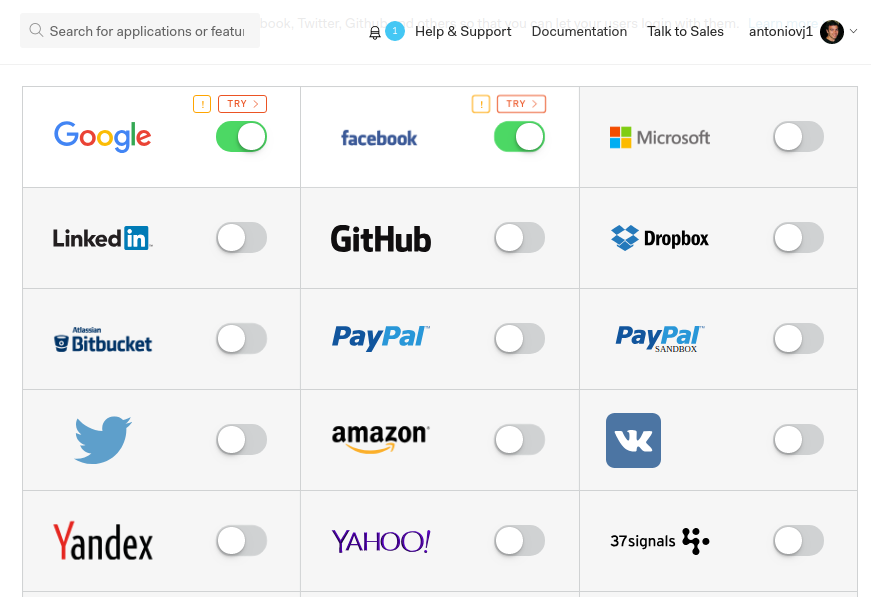
\includegraphics[width=0.95\textwidth]{imagenes/auth0.png}
    \caption{Proveedores de identidad Auth0}
    \label{fig:auth0}
  \end{center}
\end{figure}

\subsection {Bases de datos}
En esta sección se comentaré uno de los grandes motivos por los que decidimos el uso de una base de datos No-SQL, MongoDB. En un principio, no sabia exactamente que datos debía almacenar, y ademas era consciente de que a lo largo del tiempo los esquemas deberían evolucionar para proporcionar nueva información. Pensando en la implementación con una base de datos SQL y tras hacer algunas pruebas, comprobé que definir unos esquemas, añadir datos y a posteriori añadir nuevas columnas al esquema o eliminar alguna de las existentes parecía una tarea bastante tediosa y por ello decidimos optar por una solución mas flexible, en la que modificar los esquemas consistiera en realizar simples modificaciones en nuestro código y olvidarnos de migraciones.

\subsection {Ecosistema de React}
El principal problema encontrado, no ha sido a nivel de código, si no a nivel de gestión de dependencias. React solo proporciona algunas funciones básicas para la gestión de los componentes y su estado. Conforme queremos ir realizando mas operaciones, debemos ir añadiendo paquetes de NPM que nos den esa funcionalidad, de modo que en este proyecto encontramos un total de 78 dependencias, de las cuales 21 son para el desarrollo. Para cada nueva funcionalidad existe numerosas alternativas y numerosas versiones en constante cambio, lo cual crea una gran dificultad para elegir y una gran inversión de tiempo en lectura de documentación para averiguar cual se ajusta mejor a nuestro problema, además de las posibles incompatibilidades de versiones entre unos paquetes y otros. Para ilustrar la complejidad, cabe decir que actualmente existen mas de 700000 paquetes en NPM.

\subsection {Hot Module Replacement}
Durante la fase de desarrollo es interesante poder visualizar los cambios con la mayor agilidad posible, en principio mediante el uso de webpack y su opción de monitorización era posible recompilar la aplicación completa con cada cambio realizado. Esto suponía dos problemas, en primer lugar, era lento, y en segundo lugar, en cada recarga se perdía el estado de la pantalla debido a la recarga. Para subsanar esta situación se hizo uso de una técnica llamada HMR (Hot Module Replacement), con la cual tras añadir una serie de configuraciones y solventar los conflictos que generaba con la configuración te test, fuimos capaces de recompilar solo las partes afectadas por los cambios y mostrarlas sin necesidad de recargar el navegador y aun más importante, sin perder el estado.









